\documentclass[12pt]{article}

\usepackage{paper,math}
\usepackage[margin=1in]{geometry}
\addbibresource{references.bib}
\usepackage{xcolor}  % To define colors like mygr
\usepackage[most]{tcolorbox}  % For colored boxes
\usepackage{tikz} 
\usepackage{algorithm}% http://ctan.org/pkg/algorithms
\usepackage{algpseudocode}% http://ctan.org/pkg/algorithmicx
\usepackage{algorithmicx}

\newcommand{\malte}[1]{\coauthorComment[Malte]{#1}}

\definecolor{gre}{RGB}{101, 191, 127}
\definecolor{gree}{RGB}{7, 135, 44}

\newtcolorbox{defin}[2][]{colback=mygr!10,enhanced,title= #2,#1,
attach boxed title to top left={xshift=-4mm},boxrule=0pt,after skip=1cm,before skip=1cm,right skip=0cm,breakable,fonttitle=\bfseries,toprule=0pt,bottomrule=0pt,rightrule=0pt,leftrule=4pt,arc=0mm,skin=enhancedlast jigsaw,sharp corners,colframe=mygr,colbacktitle=mygr,boxed title style={
	frame code={ 
		\fill[mygr](frame.south west)--(frame.north west)--(frame.north east)--([xshift=3mm]frame.east)--(frame.south east)--cycle;
		\draw[line width=1mm,mygr]([xshift=2mm]frame.north east)--([xshift=5mm]frame.east)--([xshift=2mm]frame.south east);
		
		\draw[line width=1mm,mygr]([xshift=5mm]frame.north east)--([xshift=8mm]frame.east)--([xshift=5mm]frame.south east);
		\fill[mygr!40](frame.south west)--+(4mm,-2mm)--+(4mm,2mm)--cycle;
	}
}
}

\definecolor{mygr}{HTML}{2C3338}



\title{Genomorientierte Bioinformatik \\ - \\ BamFeatures}
\author{Malte Weyrich}
\date{\today}
% Conditionally display thoughts (hide by switching to `\boolfalse`)
% \booltrue{INCLUDECOMMENTS}
\begin{document}

% Title Page -------------------------------------------------------------------
\maketitle
\begin{abstract}
Das Sequenzieren in der Bioinformatik generiert Milliarden von \textit{Reads} pro \textit{Sample}, welche mit
einem \textit{Mapper} an das \textit{Referenzgenom} aligniert werden. 
Diese Daten werden in einer \textit{Sequence Alignment Map (SAM)} Datei gespeichert und können zusätzlich in ein komprimiertes Format,
einer \textit{Binary Alignment Map (BAM)} Datei, umgewandelt werden. Anschließend können verschiedene Analysen auf
den \textit{BAM} Dateien durchgeführt werden. Die in diesem Report diskutierte \textit{JAR} liest eine gegebene
\textit{paired-end RNA-seq BAM} Datei ein und errechnet verschiedene Features, die in einer \textit{<tsv>} Datei
gespeichert werden. Die JAR wurde auf drei verschiedenen \textit{BAM} Dateien ausgeführt, um damit
anschließend die \textit{RPKM} Werte zu berechnen. Zudem wird die \textit{JAR} anhand ihrer Laufzeit und
Korrektheit analysiert.

\end{abstract}

\newpage
\tableofcontents
\newpage


% Paper ------------------------------------------------------------------------

% ------------------------------------------------------------------------------
% ------------------------------------------------------------------------------
\section{RNA-seq}\label{sec:inro}
Die Bezeichnung \textit{RNA-seq} bezieht sich auf ein bestimmtes Sequenzierprotokoll der Bioinformatik bei dem
möglichst alle exprimierten Transkripte mehrerer Samples mittels Hochdurchsatz-sequenziergeräten wie
\textit{Illumina} verarbeitet und die resultierenden \textit{Reads} in Ausgabe Dateien abgespeichert werden.
Bei \textit{Illumina} werden die extrahierten Transkripte mittels Ultraschall oder enzymatischer Fermentation in Fragmente mit ähnlicher Länge
zerstückelt und mit Adaptersequenzen und Barcodes versehen. Darauf folgt eine \textit{PCR} Amplifikation der 
Fragmente, um das Signal zu verstärken. Die amplifizierten Fragmente können nun im Sequenzierzyklus 
von \textit{Illumina}, Base für Base, gelesen werden. Dabei wird jedoch nicht das ganze Fragment gelesen, sondern
jeweils nur ca. $100BP$ (abhängig von Voreinstellung und Protokoll) beider Enden des Fragments (\textit{paired-end sequencing}).
Somit entstehen pro Fragment zwei \textit{Reads}, ein forward \textit{Read} und ein reverse \textit{Read},
welche zu einem \textit{ReadPair} zusammengefasst werden können. 
In dem Protokoll von \textit{Illumina} werden zuerst alle \textit{Reads} eines Endes aller
Fragmente gemacht, dann wird das Fragment, \textbf{vereinfacht gesagt}, auf der \textit{Flow Zelle} umgedreht (durch Replikation), wodurch 
die umgedrehten Fragmente jeweils das Komplement ihres ursprünglichen Fragments sind.
Somit sollten die \textit{Reads} eines \textit{ReadPairs} immer auf entgegengesetzte Stränge \textit{("+"/"-")}
\textit{"mappen"}. Ist bei einem Sequenzierexperiment die Ausgangskonfiguration der Fragmente bekannt, so handelt 
es sich um ein \textit{strangspezifisches} Experiment und man kann allen
\textit{Reads} einem festen Strang zuordnen, je nach dem, ob das Fragment in der Anfangskonfiguration
vom \textit{"-"} oder vom \textit{"+"} Strang kam.
Ein \textit{Mapper} würde nun solche \textit{ReadPairs} an einem \textit{Referenzgenom} \textit{mappen}
und eine (oder mehrere) \textit{SAM/BAM} Datei(en) erstellen, welche unter anderem die Koordinaten der alignierten 
\textit{Reads} basierend auf dem \textit{Referenzgenom} beinhalten. 
Die Alignment Daten dieser Datei können nun von der \textit{BamFeatures JAR} weiter annotiert werden. 


\section{Java Programm}
\begin{verbatim*}
Usage:
    java -jar bam.jar -bam <bamPath> -o <outputPath> -gtf <gtfPath> \\
                      [-frstrand <true/false>] [-lengths]
\end{verbatim*}
\subsection{Argumente}
Zusätzlich zu den vorausgesetzten Argumenten (\textit{-bam}, \textit{-o}, \textit{-gtf}) können noch \textit{-frstrand} und
\textit{-lengths} angegeben werden. 
Bei einem Strangpositiven Experiment (\textit{-frstrand true}) ist der forward \textit{Read} auf dem \textit{"+"} und der reverse \textit{Read} auf dem
\textit{"-"}. So kann die \textit{JAR} die \textit{Reads} korrekt zuordnen. 
Falls die Strangrichtung nicht angegeben ist, werden für beide \textit{Reads} jeweils beide Stränge betrachtet.
Die \textit{-lengths} Option wird für die Berechnung der \textit{RPKM} Werte benötigt. 
Ist diese Option gesetzt, so werden die für die Längennormalisierung benötigte Genlängen der kombinierten Exons jedes
Gens berechnet und in einer \textit{<tsv>} Datei gespeichert.
\begin{table}[htpb]
    \centering
    \caption{Übersicht der verwendeten \textit{BAM} Dateien}
    \label{tab:baminfo}
\begin{tabular}{r|c|c|c}
    \textbf{Spezies}   & \textbf{BAM} & \textbf{GTF} & \textbf{frstrand}\\ \hline
    Homo Sapiens & ebna\_hisat &GRCh37.75 & "+"/"true" \\
     Homo Sapiens & hes\_star & GRCh37.75 & "-"/"false"\\
     Hefe &  nookaew\_cm & R64-1-1.75 & $\times$ \\
\end{tabular}
\end{table}

\subsection{Logik}
\subsubsection{Erstellen der ReadPair Objekte}

Die Einträge der \textit{BAM} Datei werden der Reihe nach von einem \textit{SAMFilereader} eingelesen. Da es
sich um \textit{paired-end} Daten handelt, muss für jeden \textit{Read} sein zugehöriger \textit{Mate} gefunden werden. 
Reads die nicht gepaart sind, oder nicht den Qualitätsanforderungen der Aufgabenstellung entsprechen,
werden ignoriert.
\textit{Read Objekte} die zum ersten Mal vorkommen, werden in einer \\ \textit{HashMap<Id, Read> seenEntries}
gespeichert und für jede Iteration wird überprüft, ob wir die \textit{Read Id} bereits gesehen haben.
Sobald wir zwei zusammengehörende \textit{Reads} identifiziert haben, wird ein neues
\textit{ReadPair Objekt} erstellt. Dabei wird die Strangrichtung beim erstellen des Objekts berücksichtigt und
die \textit{Reads} jeweils nach \textit{forward} und \textit{reverse} kategorisiert.
Zusätzlich werden die \textit{AlignmentBlocks} beider Reads zu einem gemeinsamen \textit{Regionvector meltedBlocks} und
zwei einzelnen \textit{Regionvectors} (\textit{regionVecFw}, \textit{regionVecRw}) verschmolzen.
Dies ist notwendig für die anschlie\ss enden Berechnungen und fängt einige \textit{Edge Cases} ab.
Hat ein \textit{ReadPair} $R$ z.B. $b_{1} \in \textit{regionVecFw}, b_{2} \in \textit{regionVecRw}$ und $b_{1}.\textit{end} == b_{2}.\textit{start - X}, X > 0$,
so werden diese Blöcke verschmolzen zu: $b_{1}, b_{2} \rightarrow_{melt()} b_{neu}$, mit $b_{neu}.\textit{start} == b_{1}.\textit{start} \land b_{neu}.\textit{end} == b_{2}.\textit{end}$.
\newpage
\subsubsection{Berechnung der ReadPair Attribute}
Als erstes werden die \textit{igenes} und \textit{cgenes} berechnet:
\begin{enumerate}
    \item \textit{cgenes} := $\left\{g \in \textit{cgenes} \hspace{1mm}|\hspace{1mm} g_{start } < fwRead_{start} \land g_{end} > rwRead_{end}\right\}$
    \item \textit{igenes} := $\left\{g \in \textit{igenes} \hspace{1mm}|\hspace{1mm} g_{start} >= fwRead_{start} \land g_{end} <= rwRead_{end}\right\}$
\end{enumerate}
Für die Berechnung dieser Attribute verwenden wir ein verschachteltes Objekt \textit{intervalTreeMap} \textit{HashMap<String, HashMap<Boolean, IntervalTree<Gene>\hspace{0.1mm}>\hspace{0.1mm}>}
verwendet, welches für jedes Chromosom die Gene nach ihrem Strang in Intervalbäumen abgespeichert hat (Strang ist entweder: [\textit{true}|\textit{false}|\textit{null}]).
Falls \textit{|cgenes|} $== 0$ aber \textit{|igenes|} $> 0$  wird das \textit{ReadPair} verworfen und 
mit dem nächsten weiter gemacht, sind beide Mengen leer, so wird die kürzeste Distanz zu benachbarten Genen ausgerechnet und in
\textit{gdist} abgespeichert.
Danach wird das \textit{ReadPair} auf \textit{split-inconsistency} überprüft (Algotithmus \ref{alg:nsplit}), d.h. falls es eine überlappende 
Region beider \textit{Reads} gibt, müssen die potentiell implizierten Introns beider \textit{Reads} übereinstimmen.
\begin{algorithm}[!htbp]
    \caption{getNsplit()}\label{alg:nsplit}
\begin{algorithmic}[1]
\State \textbf{Input:} fw, rw \Comment{forward and reverse reads}
\If{$|\text{fw.Blocks}| = 1$ \textbf{and} $|\text{rw.Blocks}| = 1$}\Comment{Checks if the reads imply introns}
    \State \Return 0 
\EndIf
\State overlap = determineOverlap(fw, rw) \Comment{Determine overlap region}
\State iFwRegions $\gets \{\}$ \Comment{Set for containing fw Introns}
\State iRwRegions $\gets \{\}$ \Comment{Set for containing rw Introns}
\State iRegions $\gets \{\}$ \Comment{Set for containing all Introns}
\State \textbf{extractIntronsInOverlap}(overlap.x1, overlap.x2, iFwRegions, iRegions, fw) 
\State \textbf{extractIntronsInOverlap}(overlap.x1, overlap.x2, iRwRegions, iRegions, rw)
\If{|iRwRegions| $\neq$ |iFwRegions|}
\State \Return -1 \Comment{split-inconsistent}
\EndIf
\If{iRwRegions = iFwRegions}
\State \Return |iRegions|\Comment{Return unique Introns in overlap}
\EndIf
\State \Return -1\Comment{split-inconsistent (default)}
\end{algorithmic}
\end{algorithm}
Nach dem Aufruf von \textit{getNsplit()} wird bei einem \textit{return value} von -1 das \textit{ReadPair} als 
\textit{"split-inconsistent"} vermerkt und in die Ausgabedatei übernommen, ansonsten wird die Grö\ss e der
Menge \textit{iRegions} in der Variable \textit{nsplit} gespeichert und das \textit{ReadPair} weiter prozessiert.
\newpage
Als nächstes wird das \textit{ReadPair} anhand drei Kategorien annotiert (Abbildung\ref{fig:-figures-ReadAnnotation-png}):
\begin{figure}[htpb]
    \centering
    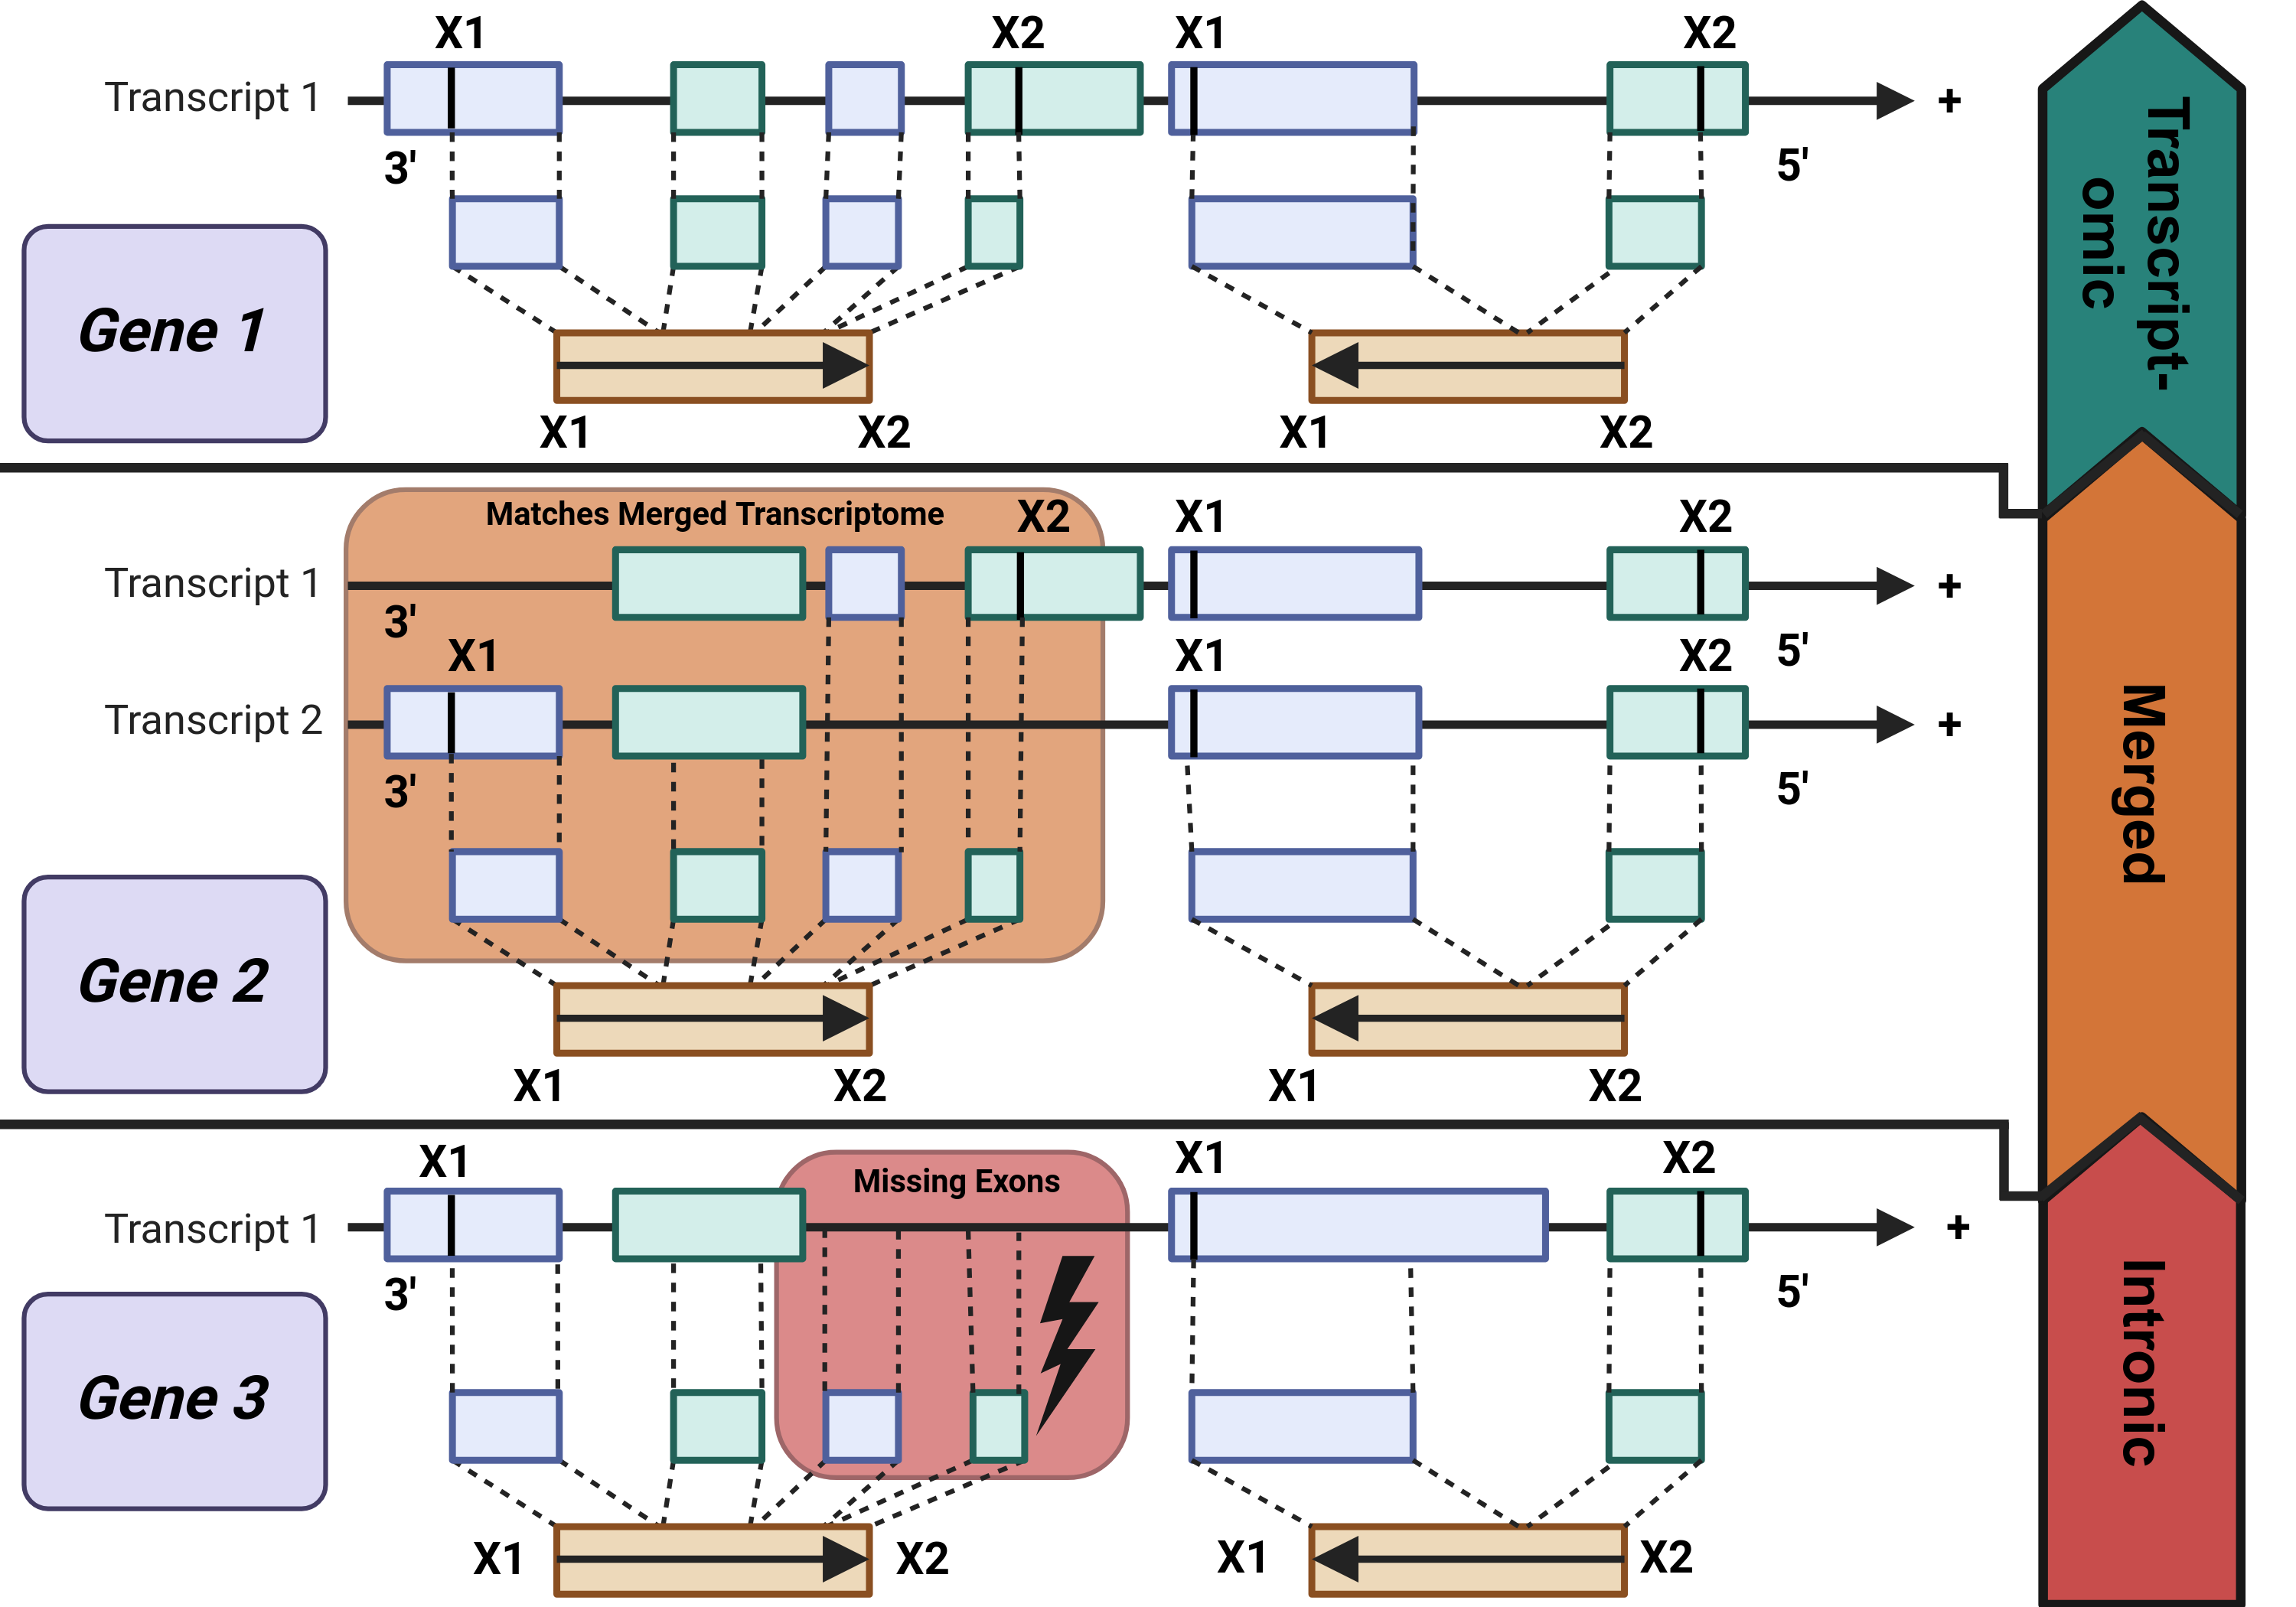
\includegraphics[width=0.95\textwidth]{./figures/ReadAnnotation.png}
\caption{Kategorisierung der \textit{ReadPair}-Regionen in die Klassen \textit{\textbf{"Transcriptomic"}},
\textit{\textbf{"Merged"}} und \textit{\textbf{"Intronic"}}, wobei eine Priorisierung nach 
der Reihenfolge \textit{\textbf{"Transcriptomic"}} > \textit{\textbf{"Merged"}} > \textit{\textbf{"Intronic"}} erfolgt.
Die \textit{AlignmentBlocks} der \textit{Reads} werden mit den Exons der Transkripte des inkludierenden Gens abgeglichen. 
Die Abbildung wurde mit \cite{biorender} erstellt.}
    \label{fig:-figures-ReadAnnotation-png}
\end{figure}

Bei der Regions-Annotation wird als erstes die \textit{\textbf{Transcriptomic}} Kategorie überprüft.
Hierbei wird über alle Gene die das \textit{ReadPair} inkludieren iteriert und für jeden \textit{Read} des \textit{ReadPairs} mit der Methode
\textit{cut(X1, X2)} zwei neuer \textit{Regionvectors} aus jedem Transkript  ausgeschnitten (Abbildung \ref{fig:-figures-ReadAnnotation-png}), 
wobei $X1$ der \textit{Alignmentstart} und $X2$ das \textit{Alignmentende} des momentanen \textit{Reads} ist.
Falls beide ausgeschnittenen \textit{Regionvectors} aus dem Transkript gleich der geschmolzenen \textit{Regionvectors} der 
\textit{Reads} entsprechen, ist das \textit{ReadPair} \textit{\textbf{Transcriptomic}} und das entsprechende Transkript
wird zusammen mit dem Gen in die Lösungsmenge genommen. 

Für die \textit{\textbf{Merged}} Kategorie reicht es, wenn die \textit{Regionvectors} der \textit{Reads} in dem geschmolzenen
Transkriptom eines Gens enthalten sind (siehe Abbildung \ref{fig:-figures-ReadAnnotation-png}). 
Das geschmolzene Transkriptom wird in Algorithmus \ref{alg:melt} berechnet und besteht aus allen annotierten Exons 
eines Gens. Wenn ein \textit{ReadPair} dieser Kategorie zugeteilt wird, wird das Gen in einer separaten Lösungsmenge
gespeichert. Falls die oberen zwei Ansätze beide nicht zutreffen, so handelt es sich um ein \textit{\textbf{Intronic}}
\textit{ReadPair}.


\begin{algorithm}[H]
\caption{Melt Exons into Regions}\label{alg:melt}
\begin{algorithmic}[1]
\State \textbf{Input:} \text{transcriptList} (list of transcripts containing exons)
\State allExons $\gets \emptyset$
\For{each transcript in transcriptList}
    \State allExons.addAll(transcript.getExonList()) \Comment{Add all exons from transcript to the list}
\EndFor
\State \text{Sort allExons by start position} \Comment{Sort exons by their start positions}
\State meltedRegions $\gets$ new TreeSet() \Comment{Create a new set for melted regions}

\If{allExons is not empty}
    \State first $\gets$ allExons.get(0) \Comment{Get the first exon}
    \State current $\gets$ new Region(first.getStart(), first.getStop()) \Comment{Create a region for the first exon}

    \For{$i \gets 1$ to $allExons.size() - 1$}
        \State exon $\gets$ allExons.get(i)
        \If{exon.getStart() $\leq$ current.getStop() + 1}
            \State current.setStop($\max$(current.getStop(), exon.getStop())) \Comment{Extend the region if exons overlap or are adjacent}
        \Else
            \State meltedRegions.add(current) \Comment{Add the completed region to the set}
            \State current $\gets$ new Region(exon.getStart(), exon.getStop()) \Comment{Start a new region}
        \EndIf
    \EndFor

    \State meltedRegions.add(current) \Comment{Add the last region}
\EndIf
\State \Return meltedRegions \Comment{Return the melted regions}
\end{algorithmic}
\end{algorithm}

Nach der Regions-Annotation wird der \textit{gcount} mit der Anzahl an annotierten Genen der 
plausibelsten Kategorie überschrieben. Als nächstes überprüft die \textit{JAR} die Anzahl an 
\textit{mismatches} der alignierten \textit{Reads} und die Anzahl an \textit{clipped bases}. 
\textit{Clipping} bedeutet, dass ein Teil des \textit{Reads} (entweder am Anfang oder am Ende) nicht 
an das \textit{Referenzgenom} aligniert werden können. Das kann mehrere Gründe haben,
z.B. kann an dem Transkript noch der \textit{Poly-A Schwanz} angebracht gewesen sein. Wenn ein
Fragment den \textit{Poly-A Schwanz} inkludiert und dieser mit sequenziert wird, so lässt sich der
Teil des \textit{Reads} nicht mehr sinnvoll \textit{mappen}.
Die Anzahl von \textit{mismatches} und \textit{clipping} sind bereits in dem \textit{Read} vermerkt
und werden lediglich für das \textit{ReadPair} aufsummiert.

Ab hier wird angefangen das Ergebnis korrekt zu formatieren.
\begin{enumerate}
    \item Falls \textit{cgenes == 0} wird die \textit{gdist} mit in das Ergebnis geschrieben.
      Wenn es sich um ein \textit{Strangpositives} oder \textit{negatives} handelt wird 
      zusätzlich auf dem \textit{Gegenstrang} nach inkludierenden Genen gesucht und bei
      einem Ergebnis grö\ss er 0 wird der Eintrag mit \textit{"antisense:true"} vermerkt.
    \item Falls \textit{cgenes > 0} wird \textit{cgenes} und die Regions-Annotation in das
        Ergebnis übernommen.
\end{enumerate}
Als letztes wird in beiden Fällen noch der \textit{pcr-index} berechnet und mit in das Ergebnis geschrieben.
Der \textit{pcr-index} speichert wie of wir ein \textit{ReadPair} bereits gesehen haben.
Wie in \ref{sec:inro} beschrieben, werden die Fragmente auf der \textit{Flow Zelle} zuerst durch \textit{PCR}
amplifiziert. Dieses Protokoll garantiert nicht eine gleichmä\ss ig starke Amplifikation über allen
Fragmenten. Viel mehr kommt es zu starken Diskrepanzen zwischen der Häufigkeit der einzelnen Fragmente. 
Der \textit{pcr-index} benutzt die \textit{meltedBlocks} der \textit{ReadPairs} als eindeutige Erkennungssignatur 
und zählt wie oft ein \textit{ReadPair} bereits vorgekommen ist.

Das Ergebnis wir mit einem \textit{BufferedWriter} in die Ergebnisdatei geschrieben und es wird mit dem nächsten 
\textit{ReadPair} weiter gemacht.

\subsubsection{Reduktion der Heap Benutzung}
Die \textit{Reads} innerhalb der \textit{BAM} sind nach Startposition sortiert. 
Dies lässt sich ausnutzen um die Arbeitsspeichernutzung zu reduzieren. Sobald
ein neues Chromosom in der \textit{BAM} Datei erreicht ist, wird die \textit{seenEntries} \textit{HashMap}
geleert. Zusätzlich wird der zu dem alten Chromosom zugehörige \textit{IntervalTree} mit dessen 
Genen gelöscht und der \textit{pcr-index} ebenfalls neu initialisiert.
\subsection{Korrektheit}

\section{Ergebnisse}
Für die drei vorgegebenen \textit{BAM} Dateien  wurden die \textit{RPKM} Werte berechnet
und in Abbildung \ref{fig:density} aufgetragen. Dafür wurde folgende Formel verwendet:
\[
    RPKM = \frac{R_{G}}{\frac{G_{L}}{1000} \cdot S}
\]
Dabei ist $R_{G}$ die Anzahl an \textit{Reads} deren Regions-Annotation auf $G$ verweist,
$G_{L}$ ist die Länge der aufsummierten geschmolzenen Exons des Gens $G$ und $S$ ist der
Skalierungsfaktor $\Big(\frac{|R_{total}|}{1000000}\Big)$.

\begin{figure}[htpb]
    \centering
    \begin{minipage}[t]{0.32\textwidth}
        \centering
        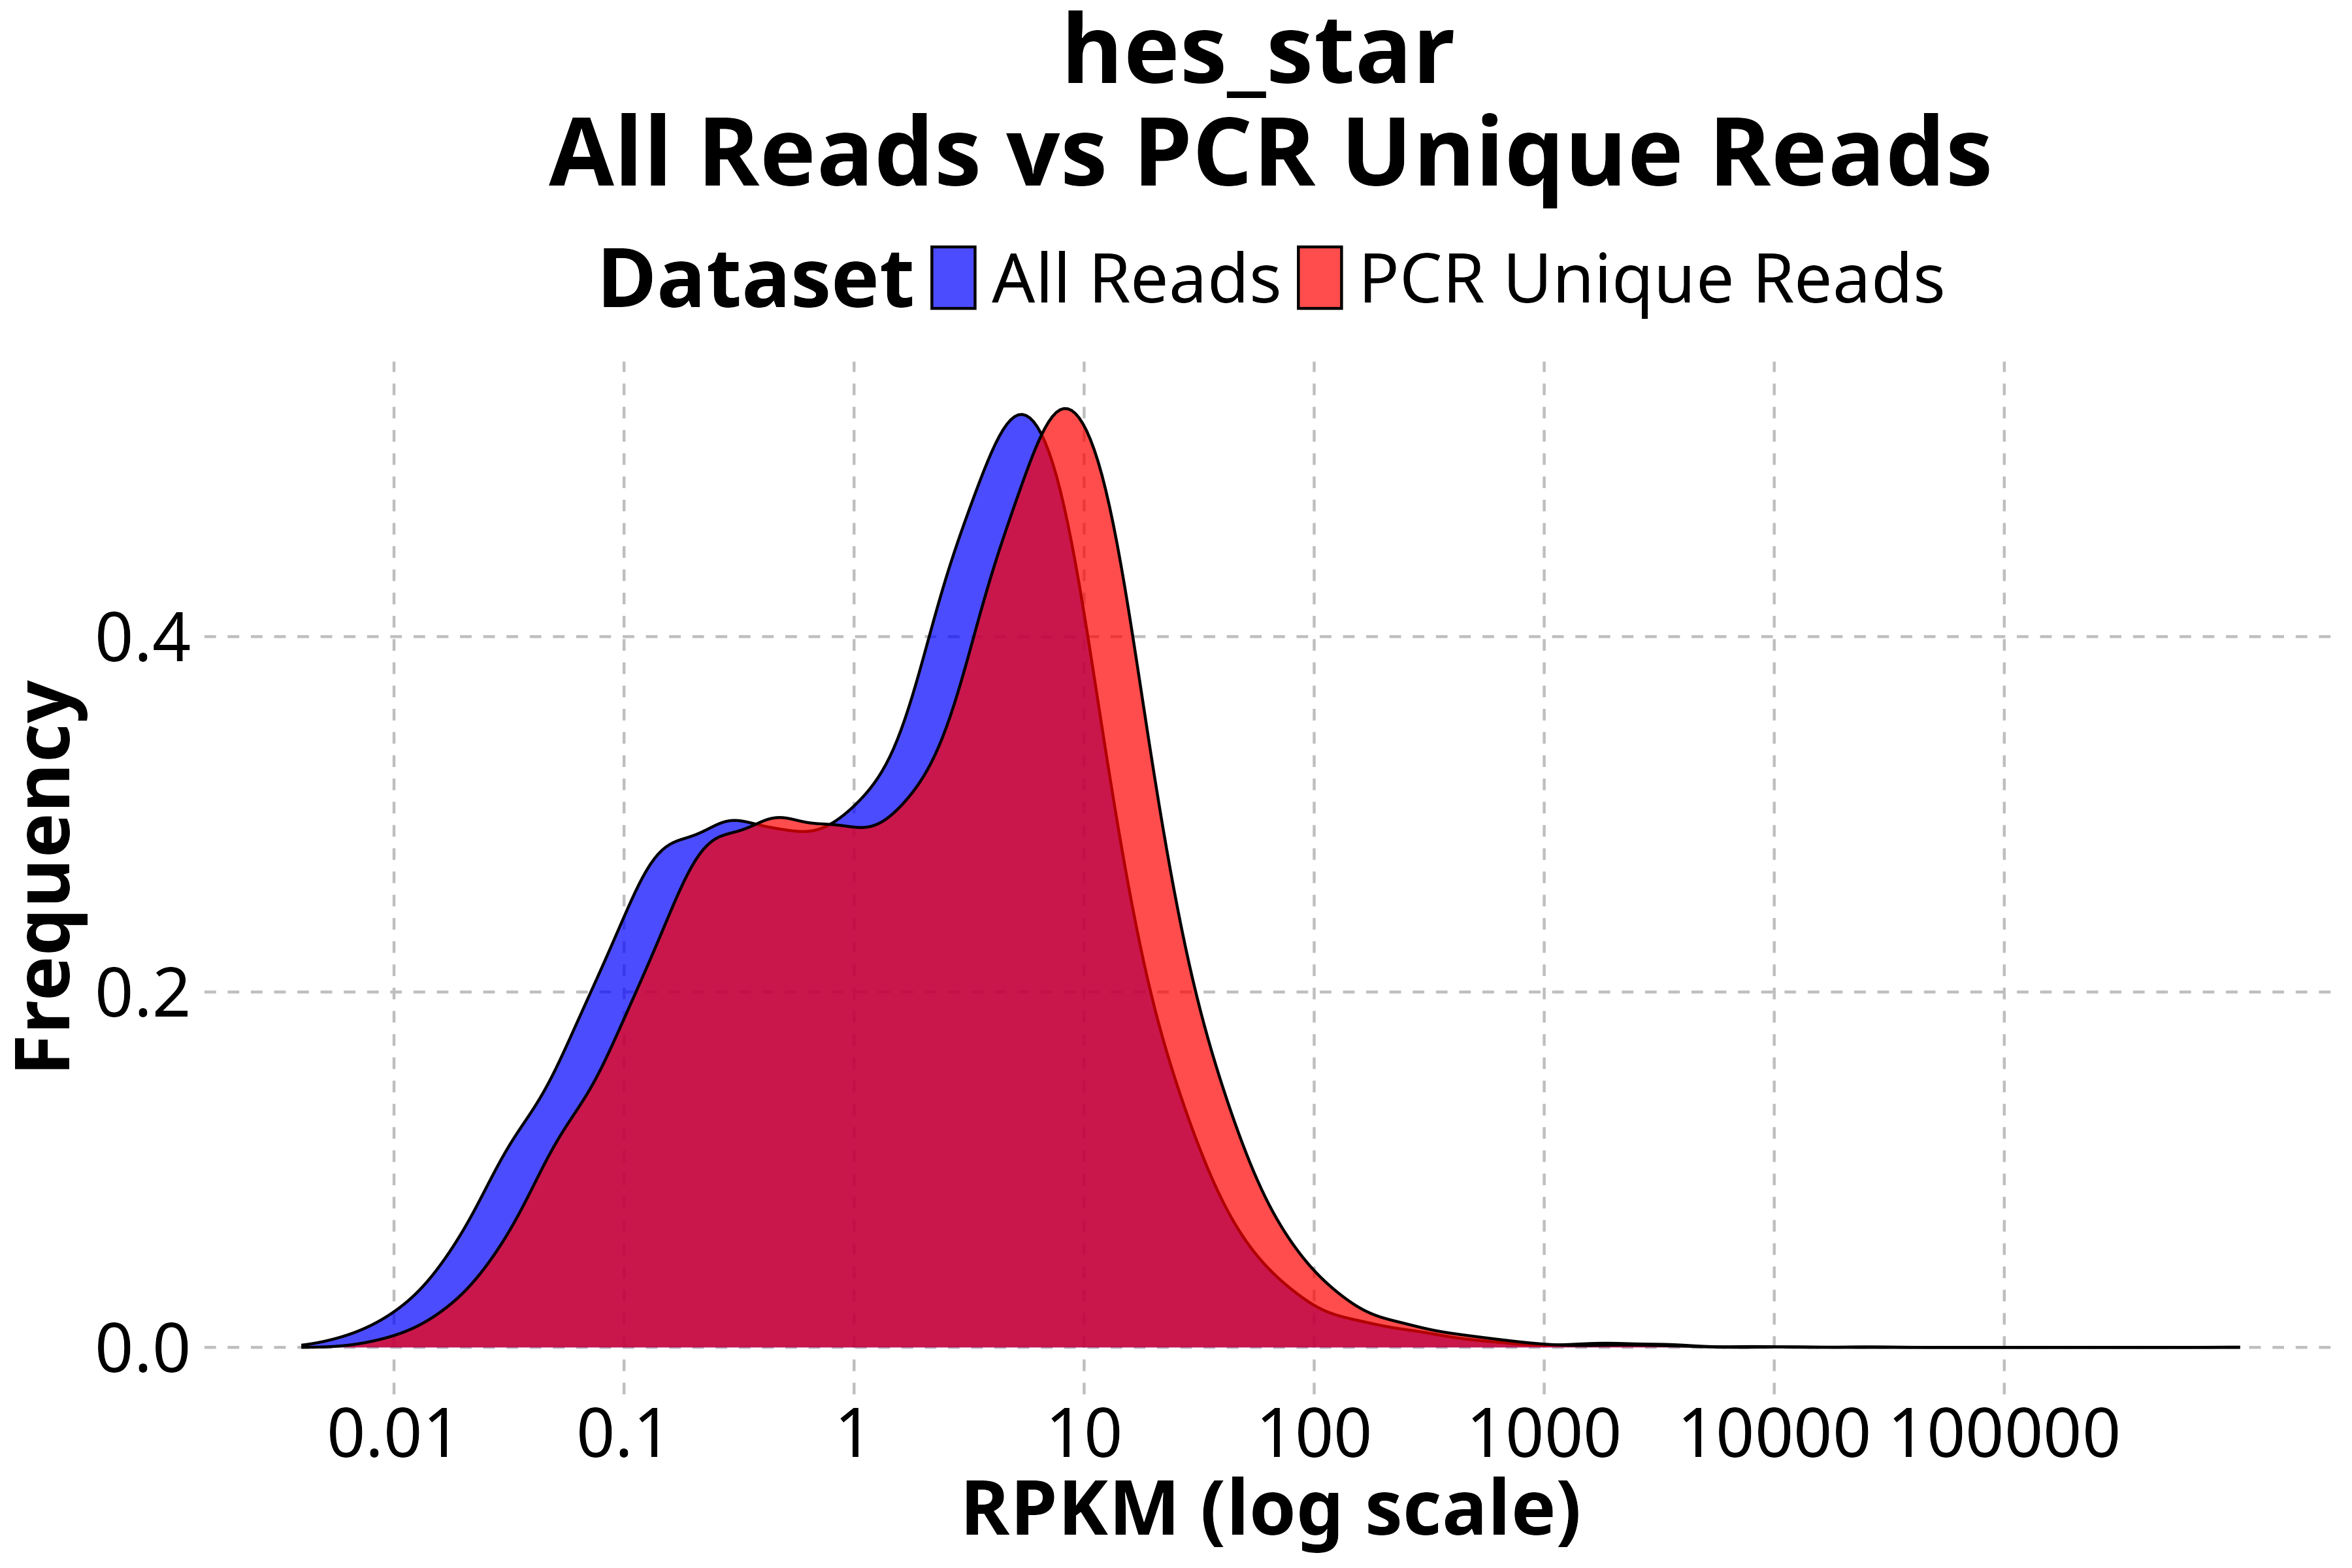
\includegraphics[width=\textwidth]{./plots/hes_star/Plots/rpkm_density.png}
    \end{minipage}%
    \hfill
    \begin{minipage}[t]{0.32\textwidth}
        \centering
        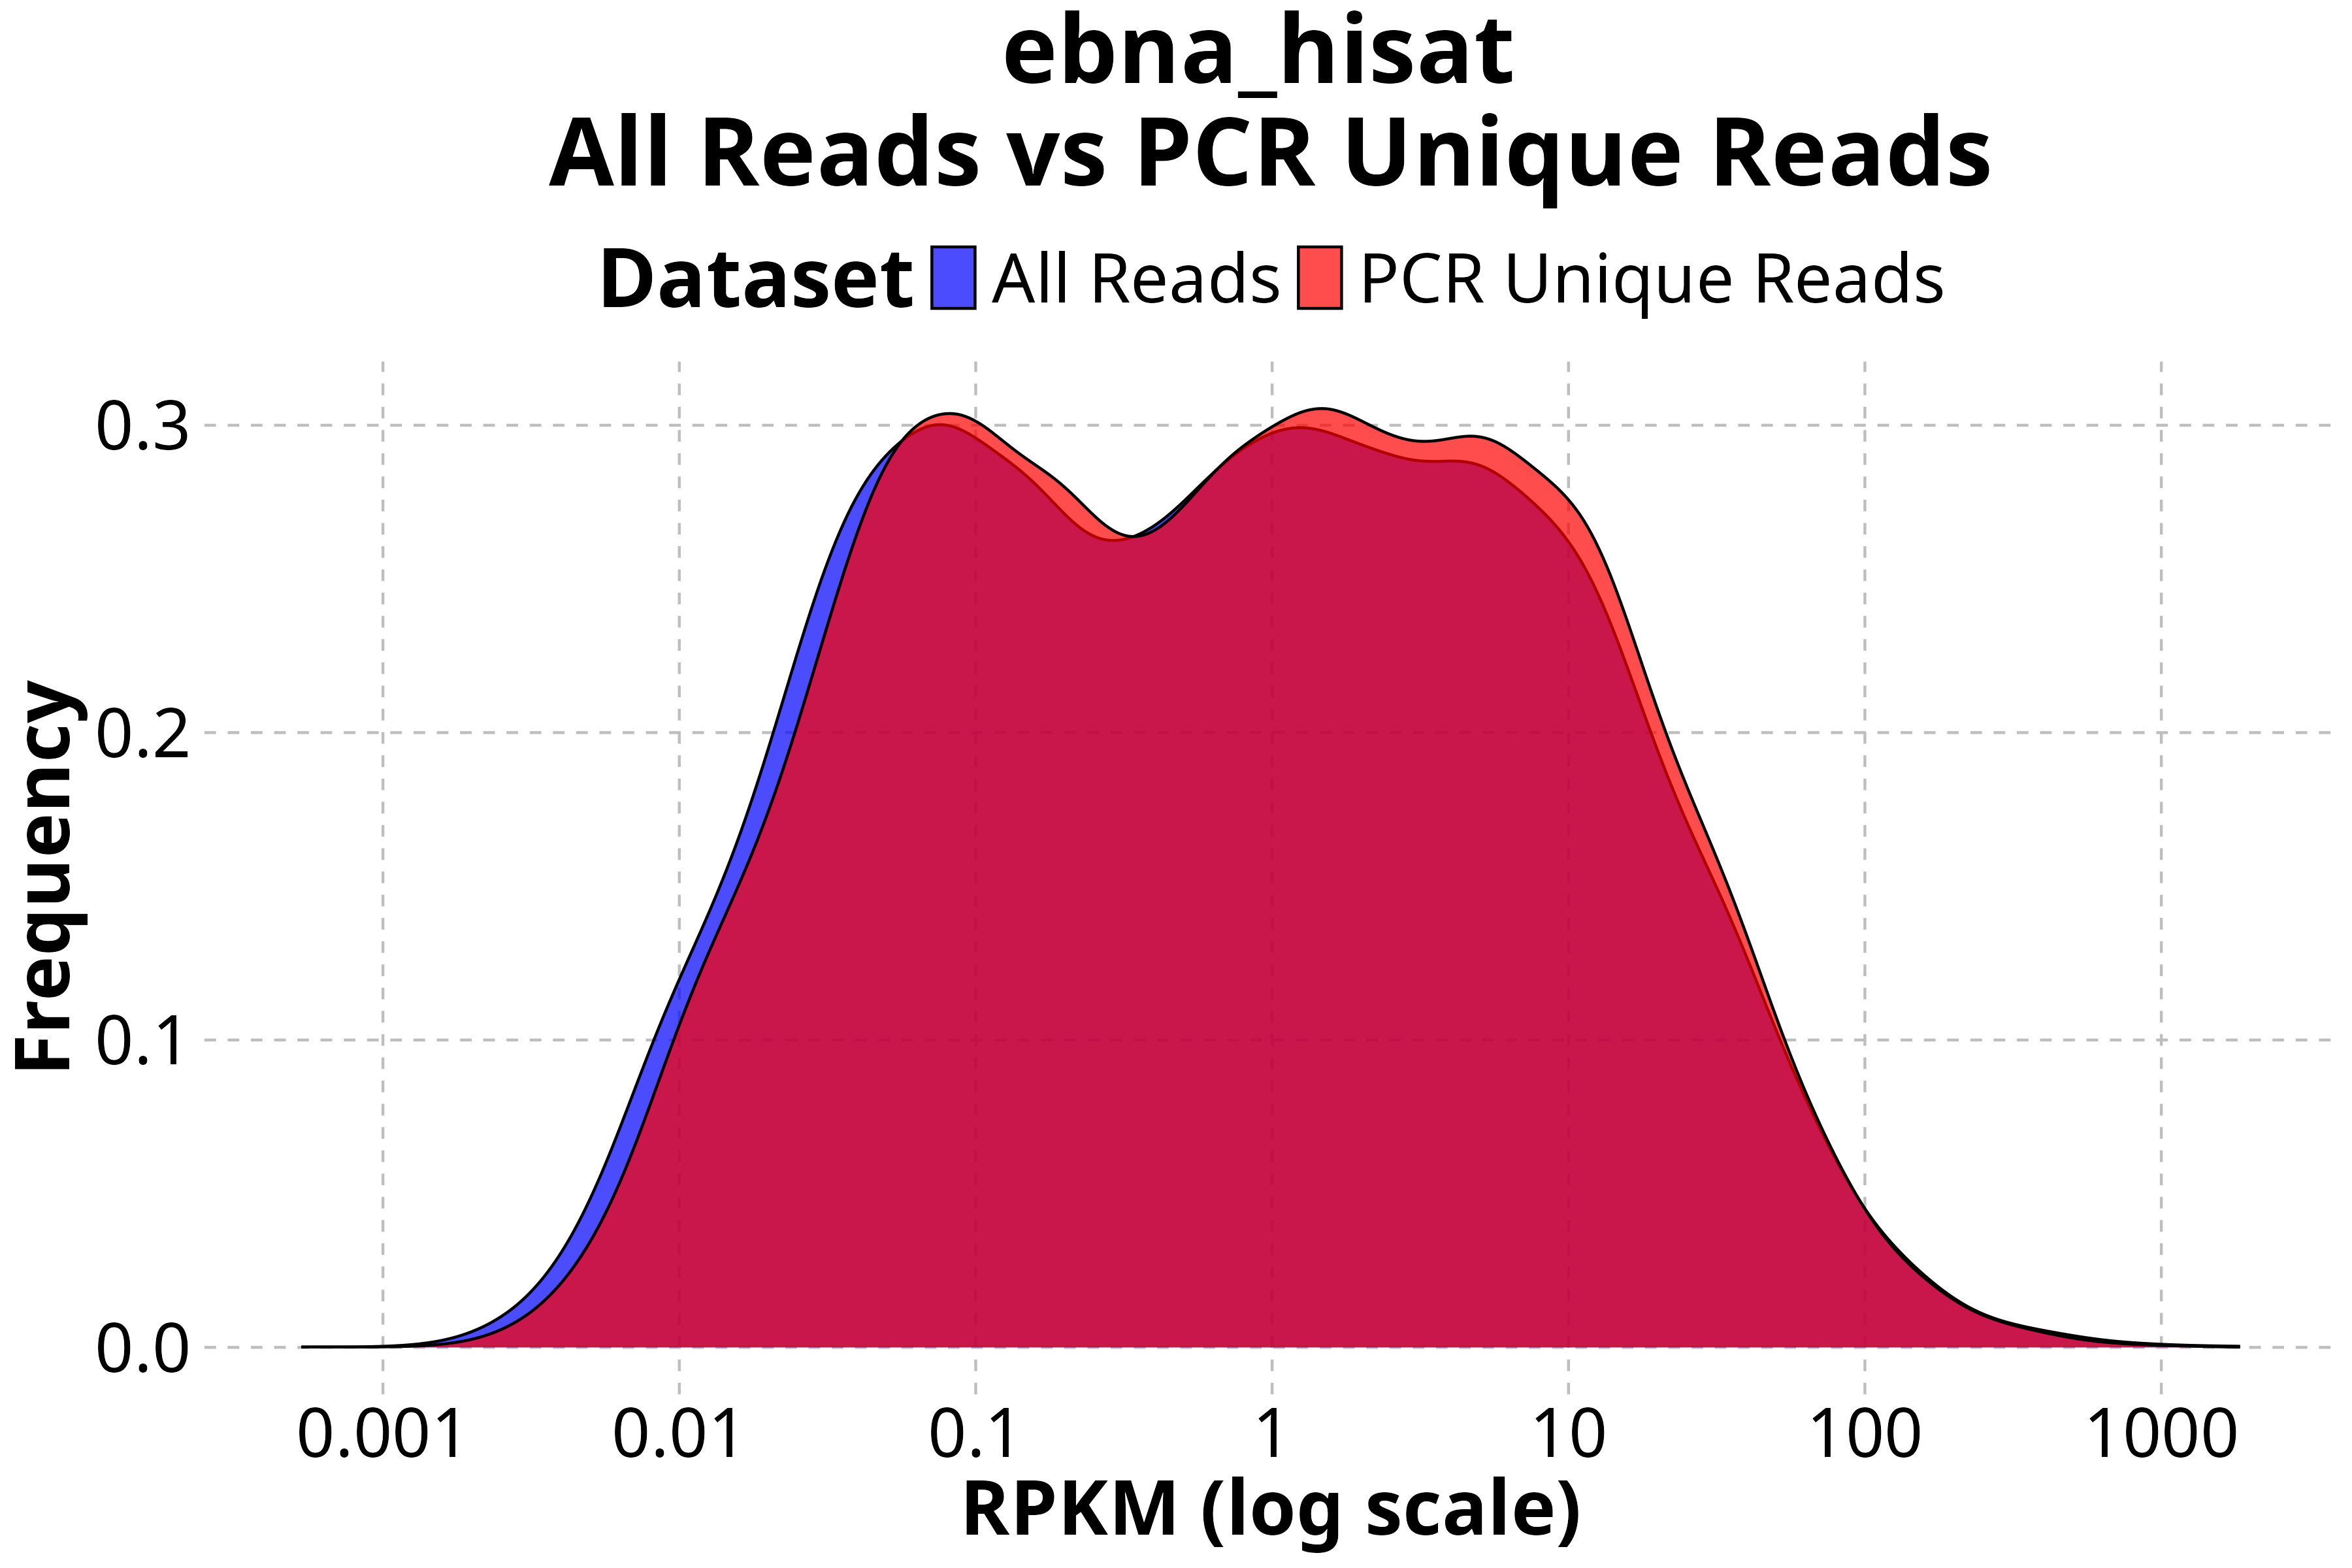
\includegraphics[width=\textwidth]{./plots/ebna_hisat/Plots/rpkm_density.png}
    \end{minipage}%
    \hfill
    \begin{minipage}[t]{0.32\textwidth}
        \centering
        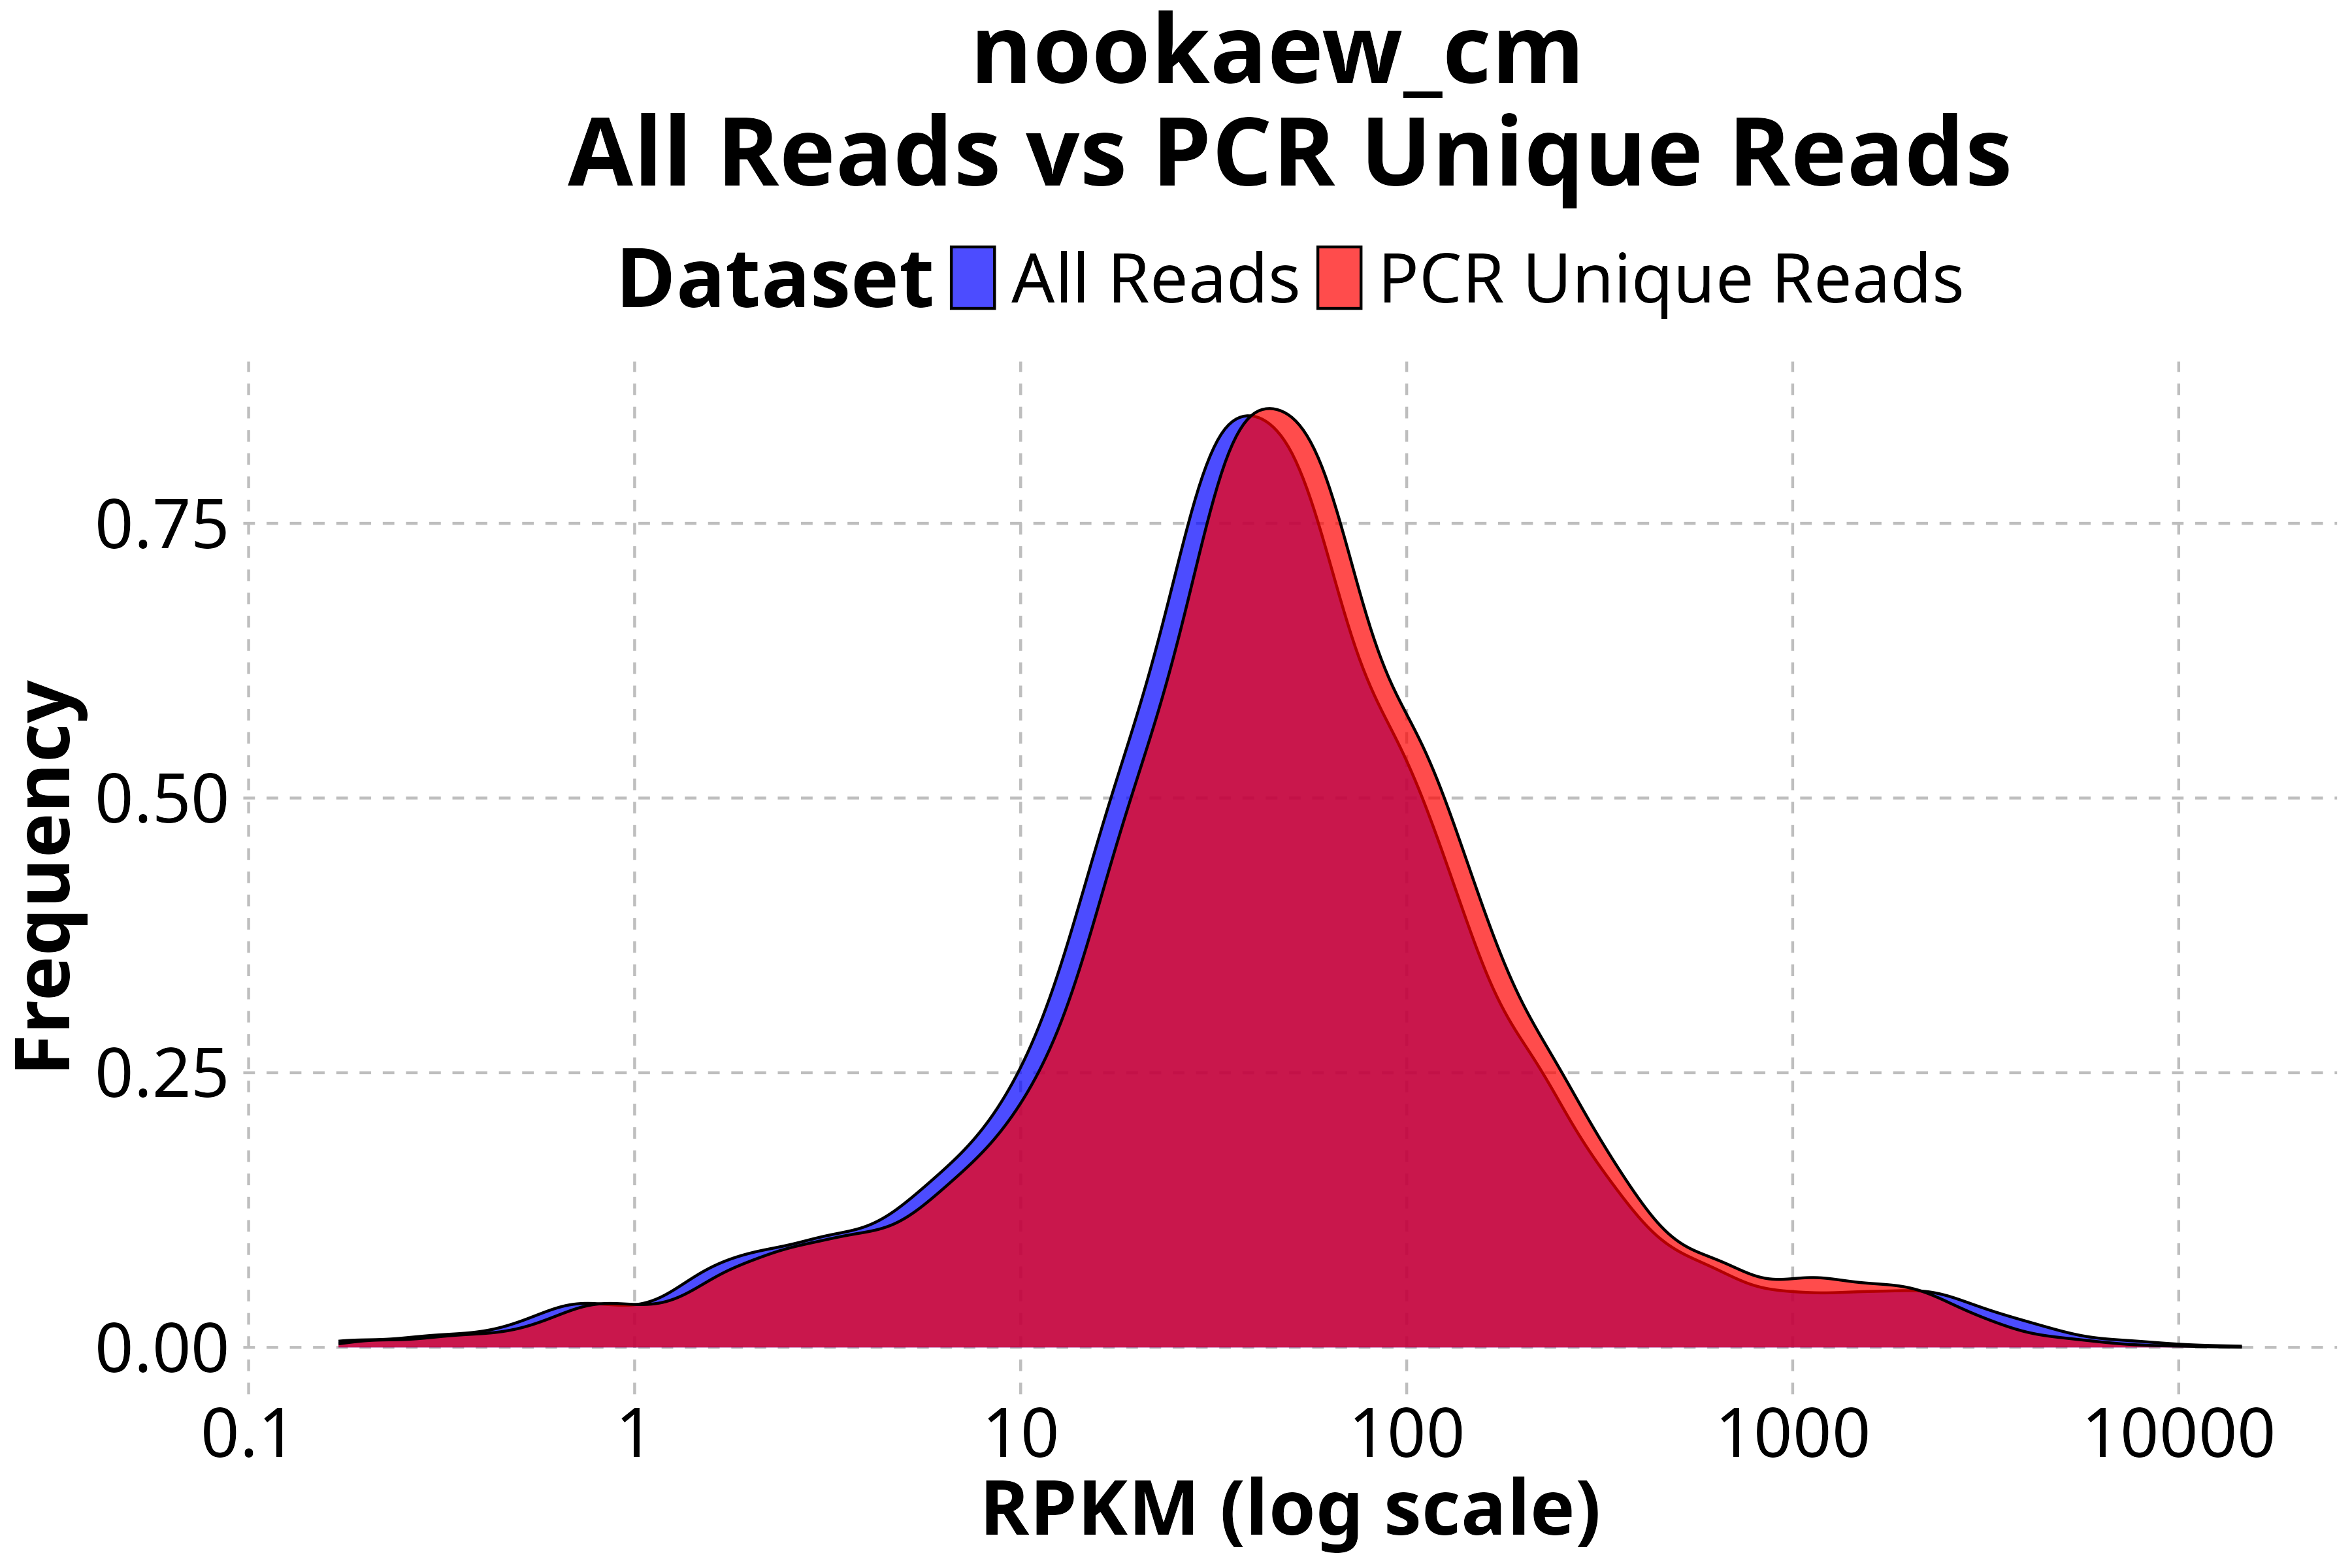
\includegraphics[width=\textwidth]{./plots/nookaew_cm/Plots/rpkm_density.png}
    \end{minipage}
    \caption{RPKM Verteilung der Gene per Sample. Dabei wird zwischen \textit{All Reads} und \textit{PCR unique Reads} unteschieden.
    \textit{All Reads} inkludiert alle \textit{ReadPairs} die eine Regions-Annotation besitzen. Bei \textit{PCR unique Reads} 
    werden nur \textit{ReadPairs} mit \textit{pcr-index = 0} berücksichtigt.}
    \label{fig:density}
\end{figure}

\begin{figure}[htpb]
    \centering
    \begin{minipage}{0.48\textwidth}
        \centering
        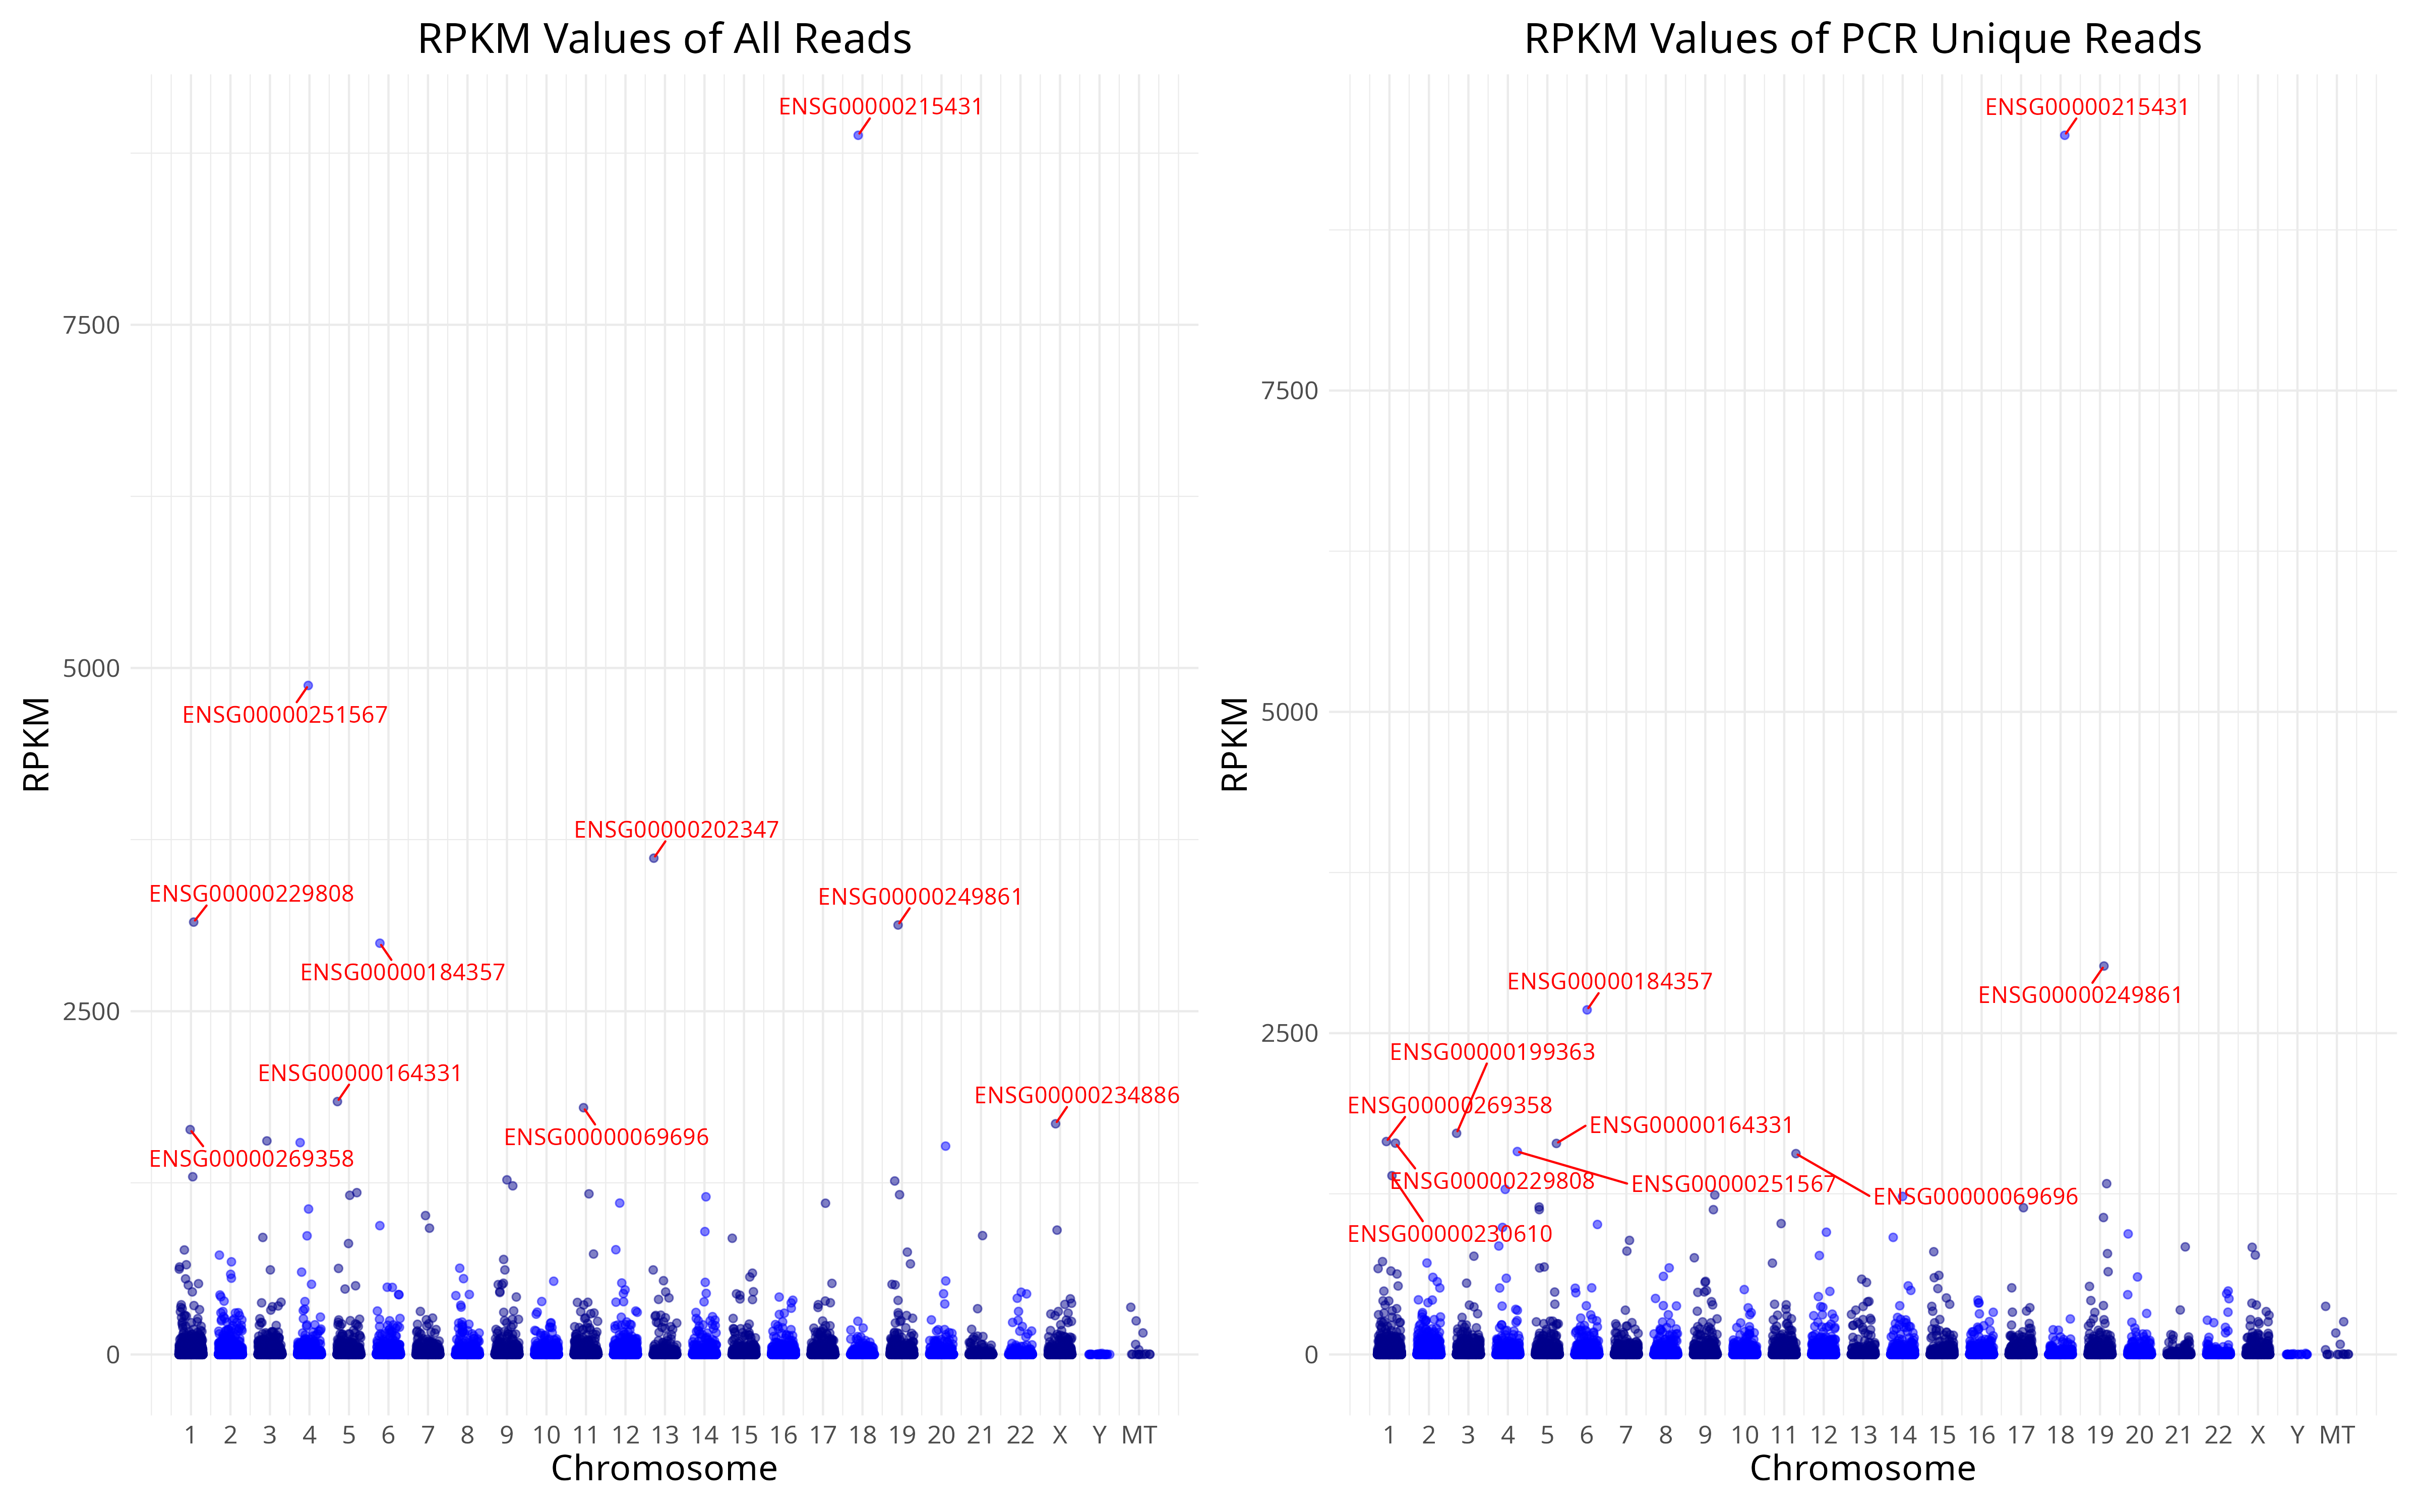
\includegraphics[width=\textwidth]{./plots/ebna_hisat/Plots/rpkm_mplot.png}
    \end{minipage}
    \hfill
    \begin{minipage}{0.48\textwidth}
        \centering
        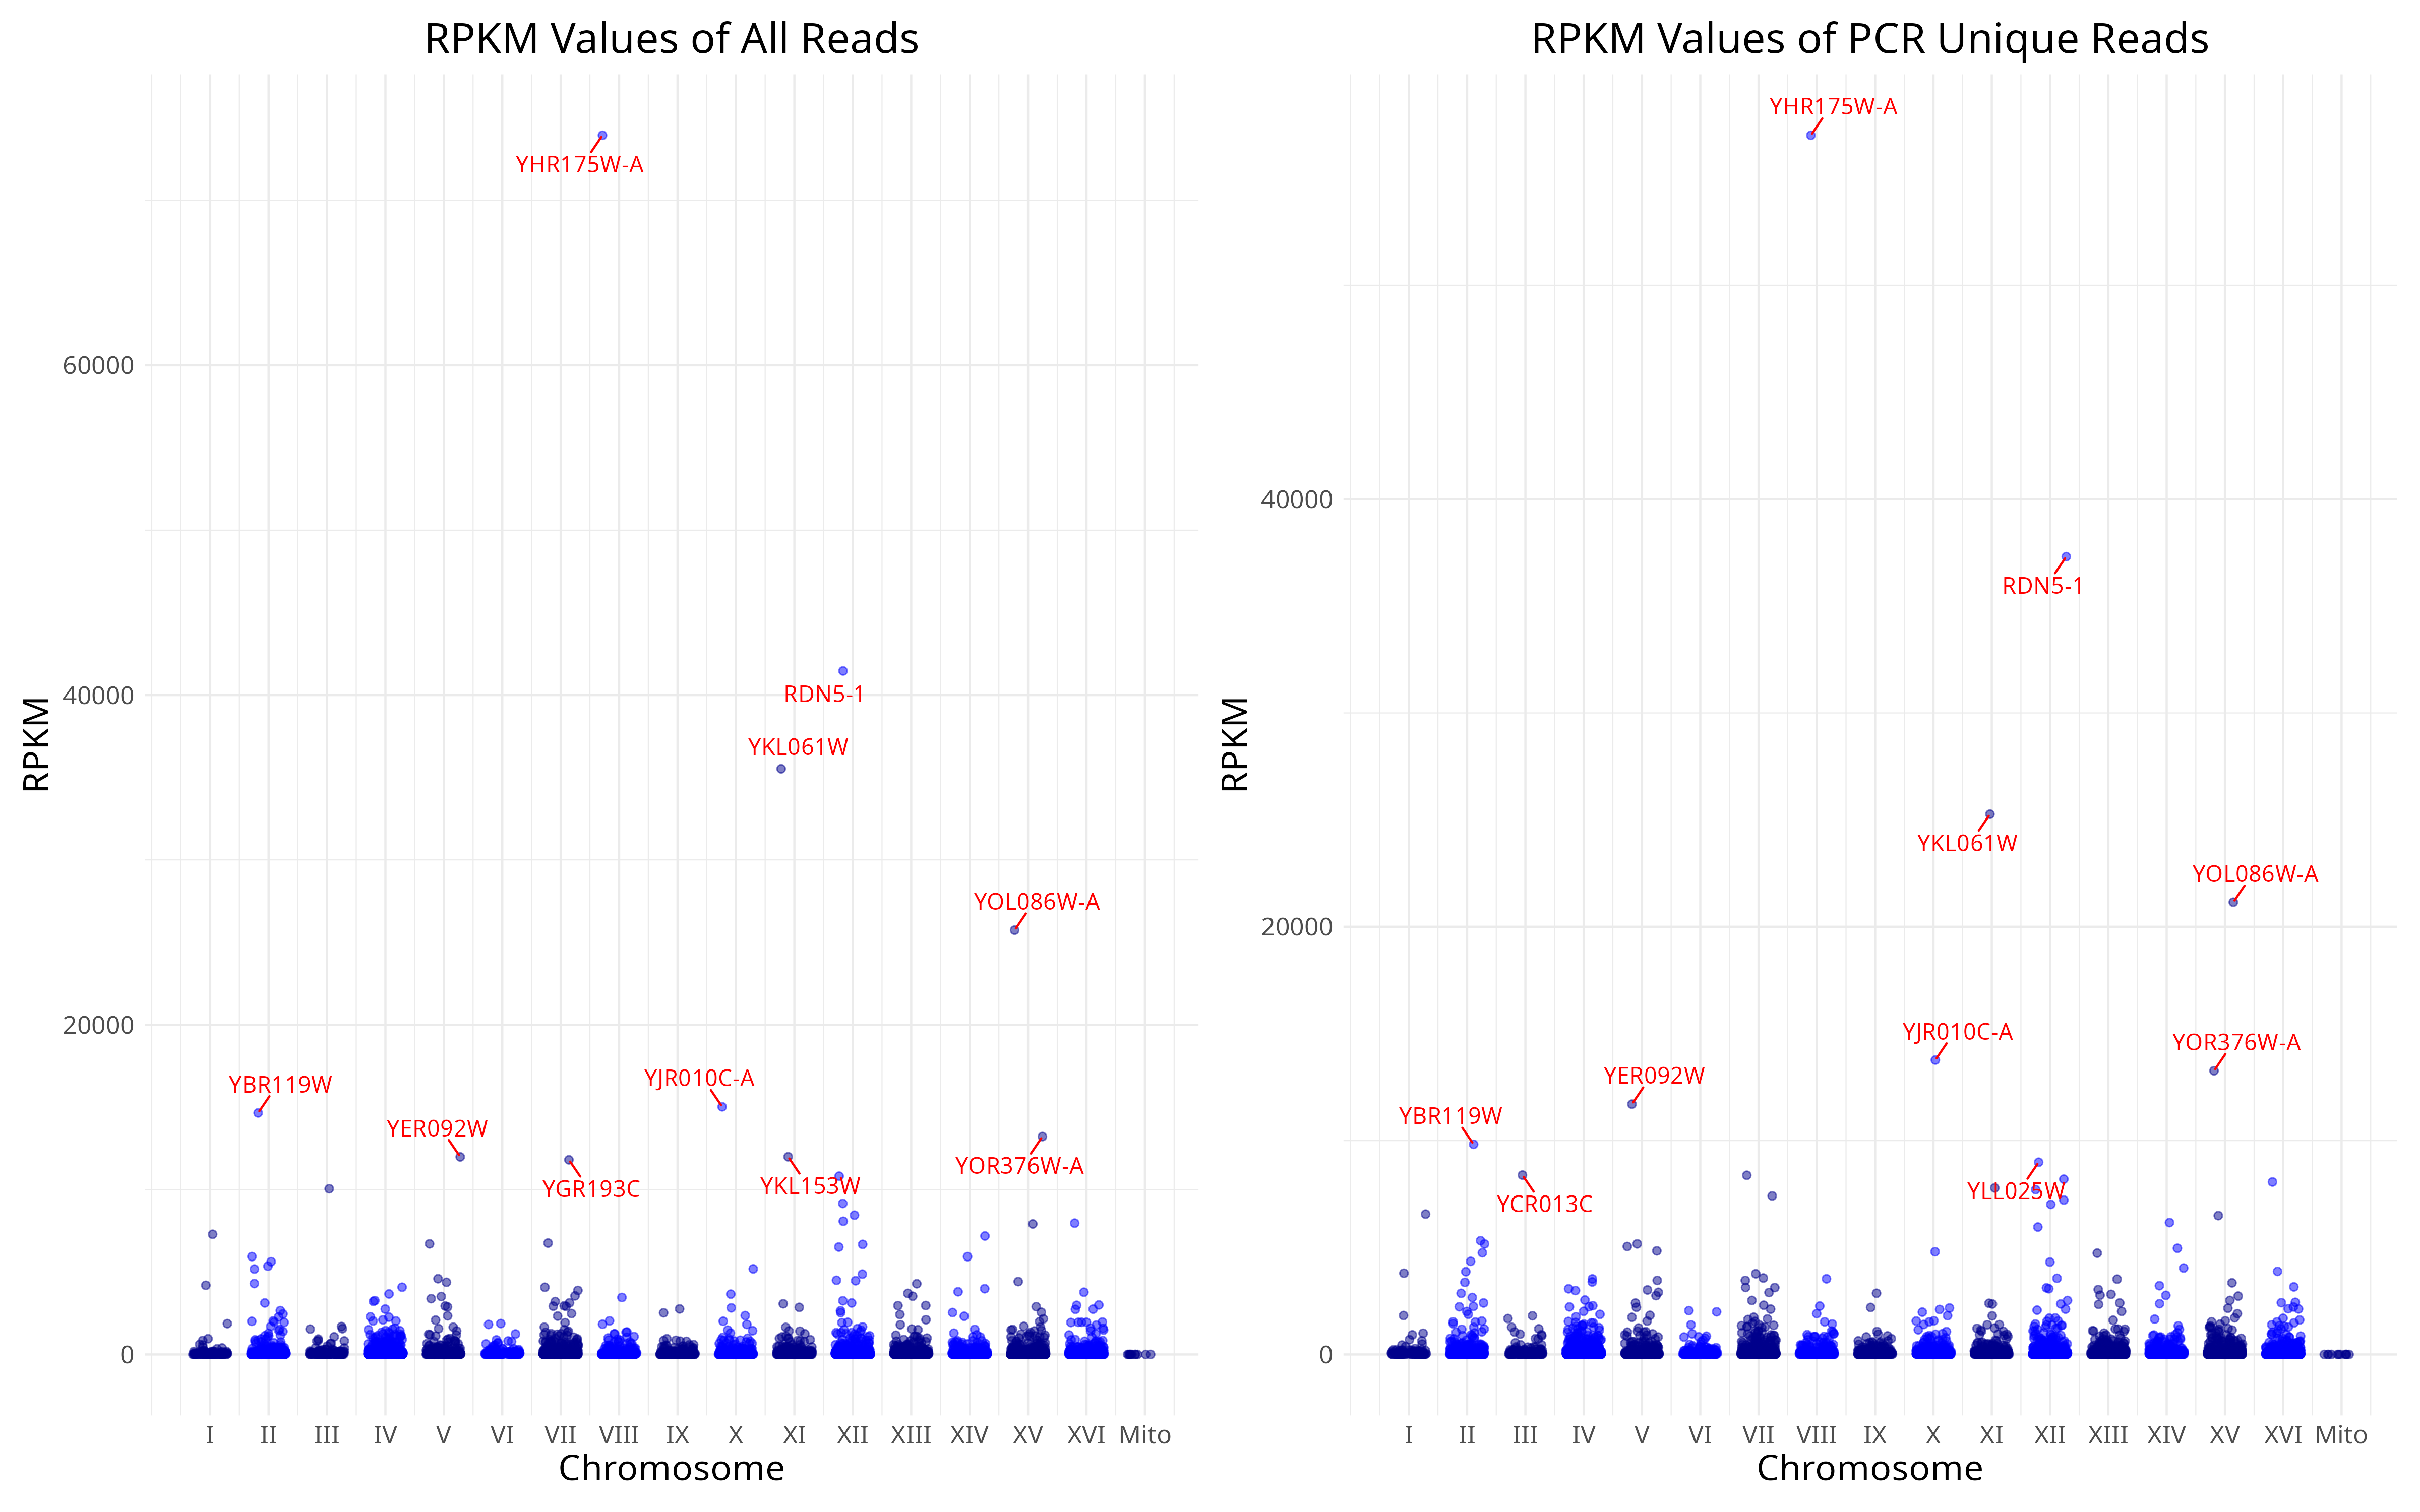
\includegraphics[width=\textwidth]{./plots/nookaew_cm/Plots/rpkm_mplot.png}
    \end{minipage}
    \caption{}
\end{figure}

\begin{figure}[htpb]
    \centering
    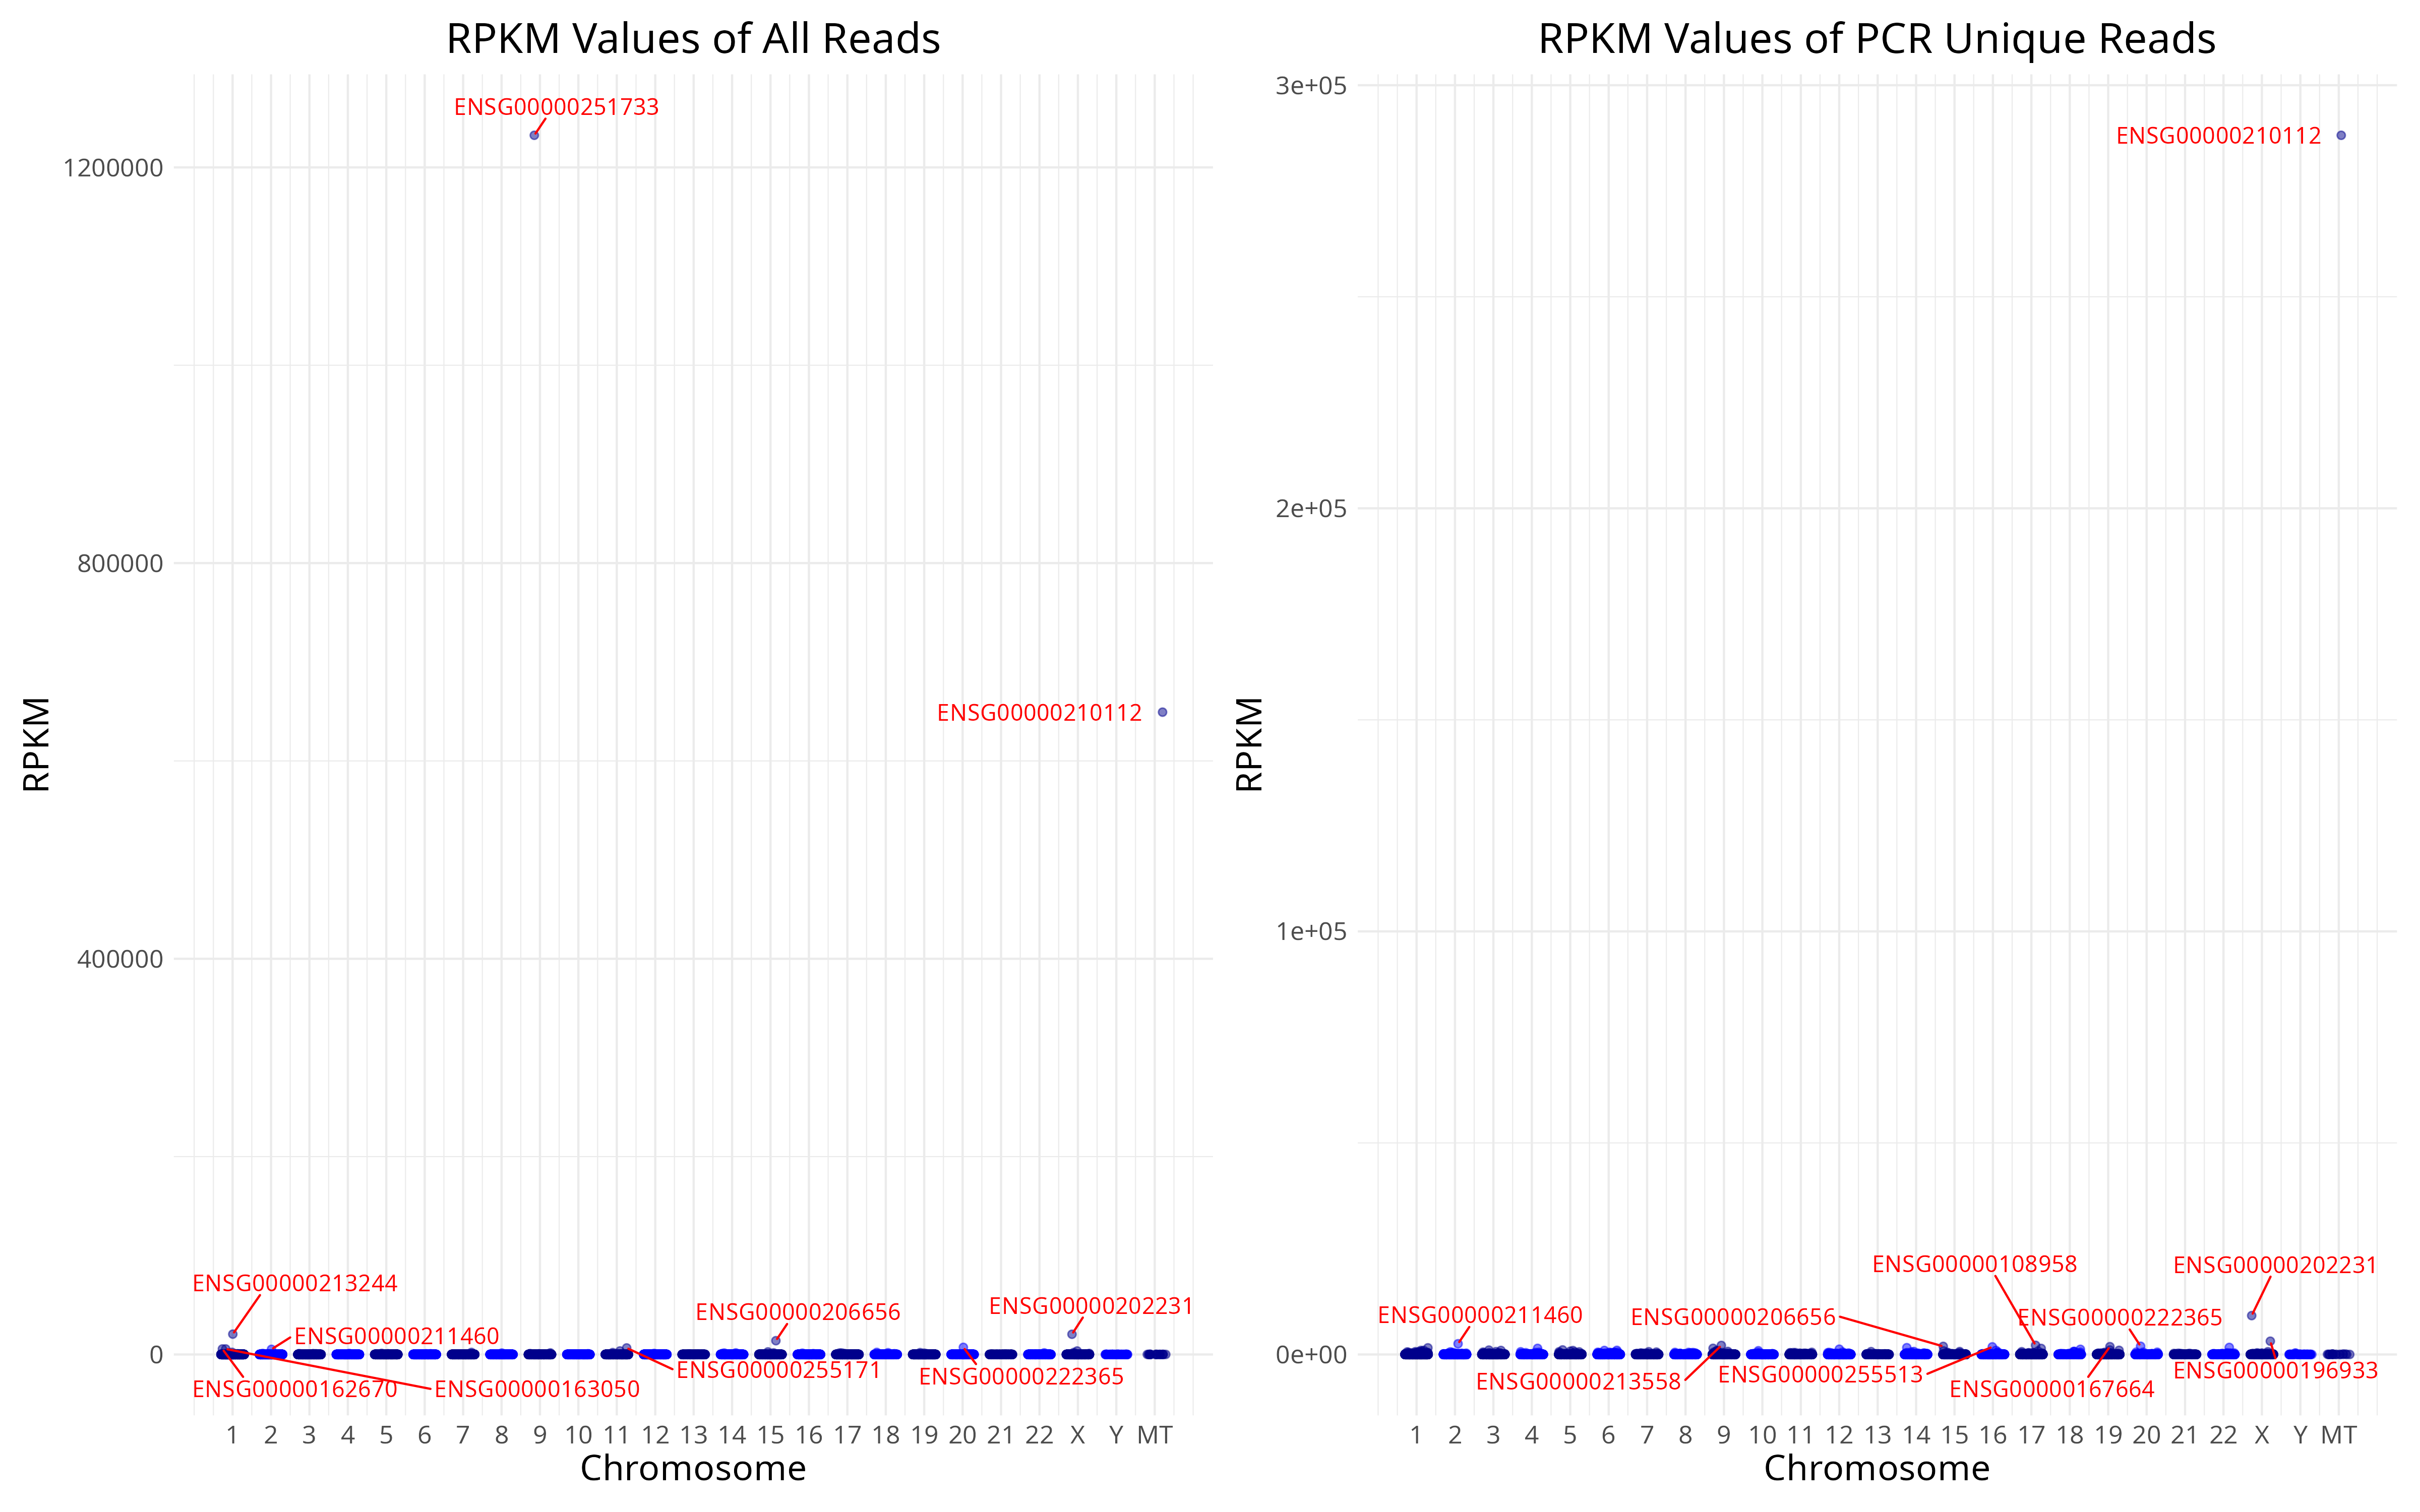
\includegraphics[width=0.85\textwidth]{./plots/hes_star/Plots/rpkm_mplot.png}
    \caption{}
    \label{fig:-plots-hes_star-Plots-rpkm_mplot-png}
\end{figure}

\subsection{Laufzeit}\label{sec:laufzeit}
Die Komplexität der \textit{JAR} ist linear in der Anzahl an Einträgen der \textit{BAM} Datei und der \textit{GTF}-Datei,
wobei das Einlesen der \textit{GTF-Datei}, bei gro\ss en \textit{BAM} Dateien,  nur einen Bruchteil $G$ der Gesamtkosten ausmacht.
Im worst case sind alle \textit{Reads} in einer \textit{BAM}-Datei mit $R$ vielen Einträgen valide. Somit gibt es insgesamt 
$\frac{R}{2}$ viele \textit{ReadPairs} welche im worst case alle \textit{genic} sind, d.h eine Regions-Annotation haben.
Für jeden dieser \textit{ReadPairs} kostet die gesamte Annotation $K$ viel Aufwand, wobei dieser Aufwand konstant ist.
Somit beträgt die Laufzeit im worst case:
\[
    \mathcal{O}(G + R + \frac{R}{2} \cdot K) \in \mathcal{O}(G + 2 \cdot R \cdot K) \in \mathcal{O}(G+R) \in \mathcal{O}(R)
.\]
Da $G <<< R$ für gro\ss e \textit{BAM} Dateien.
\subsection{Benchmarking}
Die in \ref{sec:laufzeit} theoretisch bestimmte Laufzeit spiegelt sich in Abbildung \ref{fig:-plots-times_bam-jpg} wieder.
Wenn man zusätzlich die Anzahl an annotierten \textit{ReadPairs} in Tabelle \ref{tab:amount} betrachtet, lässt sich grob 
abschätzen, dass die \textit{JAR} pro $20$ Mio \textit{ReadPairs} ca. $200s$ braucht. Sie skaliert sogar etwas besser
für noch grö\ss ere Dateien, denn für $>46$ Mio \textit{ReadPairs} in der \textit{ebna\_hisat} Datei benötigt sie 
unter $400s$.

\begin{figure}[htpb]
    \centering
    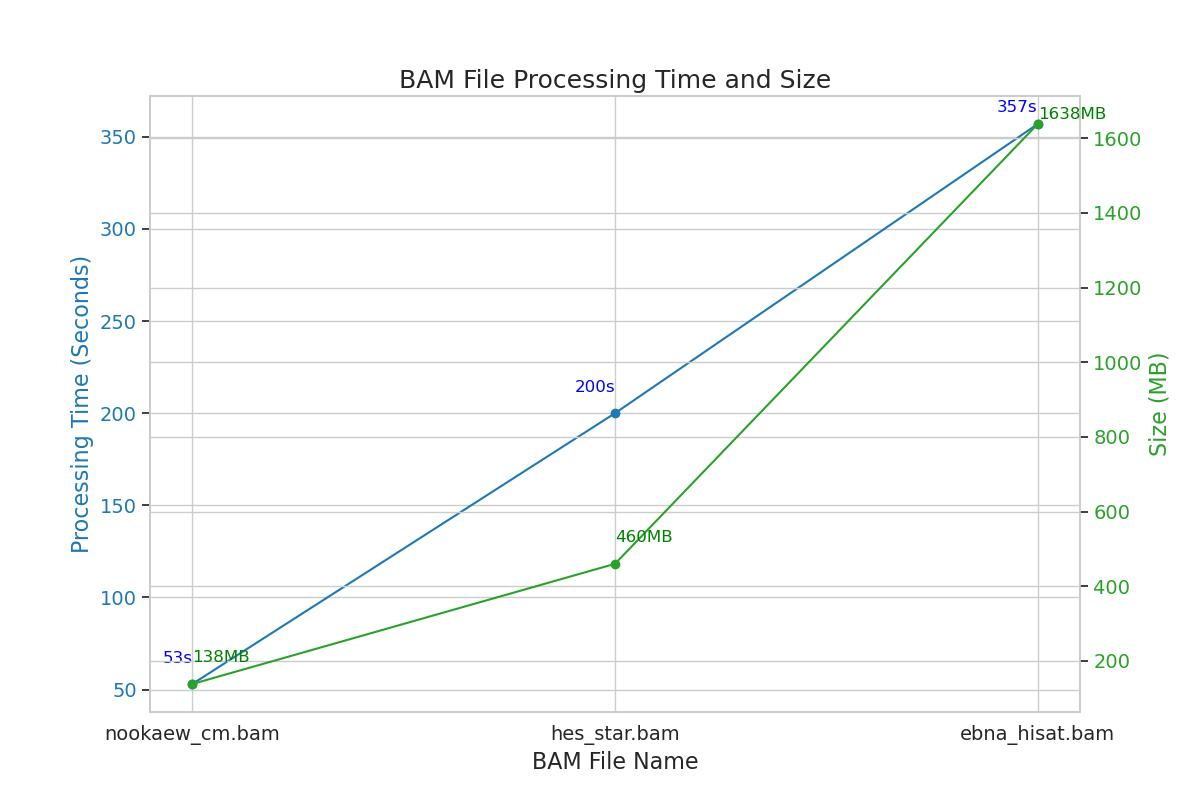
\includegraphics[width=0.7\textwidth]{./plots/times_bam.jpg}
    \caption{Laufzeit der JAR auf den 3 vorgegebenen \textit{BAMs} in Sekunden verglichen mit dem \textit{BAM} Volumen in \textit{MB}. 
    Die Ausführung der JAR erfolgte auf folgender Hardware (CiP Rechner): Intel(R) Core(TM) i7-8700 CPU @ 3.20GHz mit 6 Kernen (12 Threads), 12 MB L3-Cache, und einer RAM-Limitation von 10 GB (-Xmx10g). }
    \label{fig:-plots-times_bam-jpg}
\end{figure}

\begin{table}[htpb]
    \centering
    \caption{Anzahl an annotierten \textit{ReadPairs} per \textit{BAM} Datei}
    \label{tab:amount}

    \begin{tabular}{r|l}
        \textbf{BAM} & \textbf{Total \textit{ReadPairs}} \\ \hline
          ebna\_hisat   & 46536090 \\
          hes\_star    & 20098529 \\
          nookaew\_cm    &  5054624 \\
    \end{tabular}
\end{table}






% ------------------------------------------------------------------------------
\newpage
\printbibliography
% ------------------------------------------------------------------------------


% ------------------------------------------------------------------------------
% \newpage~\appendix
% ------------------------------------------------------------------------------



\end{document}
